\section{Introduction}
\label{sec:introduction}

% state the learning objective
\paragraph{} 
The objective of this laboratory assignment is to study a circuit containing a voltage source $V_A$, a current-controlled voltage source $V_C$, a current source $I_D$ and a voltage-controlled current source $I_B$ connected to different fixed value resistors $R_1$, $R_2$, $R_3$, $R_4$, $R_5$, $R_6$ and $R_7$. The circuit can be seen in Figure~\ref{fig:circuit}.

\paragraph{}
In Section~\ref{sec:theoretical}, a theoretical introduction is made in order to contextualize all the main principles that sustain our analysis of the circuit. This circuit is carefully analysed according to two of the most efficient ways to solve a circuit: the Mesh Current Method and the Node Voltage Method, both presented in Section~\ref{sec:analysis}. In Section~\ref{sec:simulation}, the circuit is analysed by simulation and the results are compared to the theoretical results obtained in Section~\ref{sec:analysis}. The conclusions of this study are outlined in the final part of the report, in Section~\ref{sec:conclusion}.

\begin{figure}[h] \centering
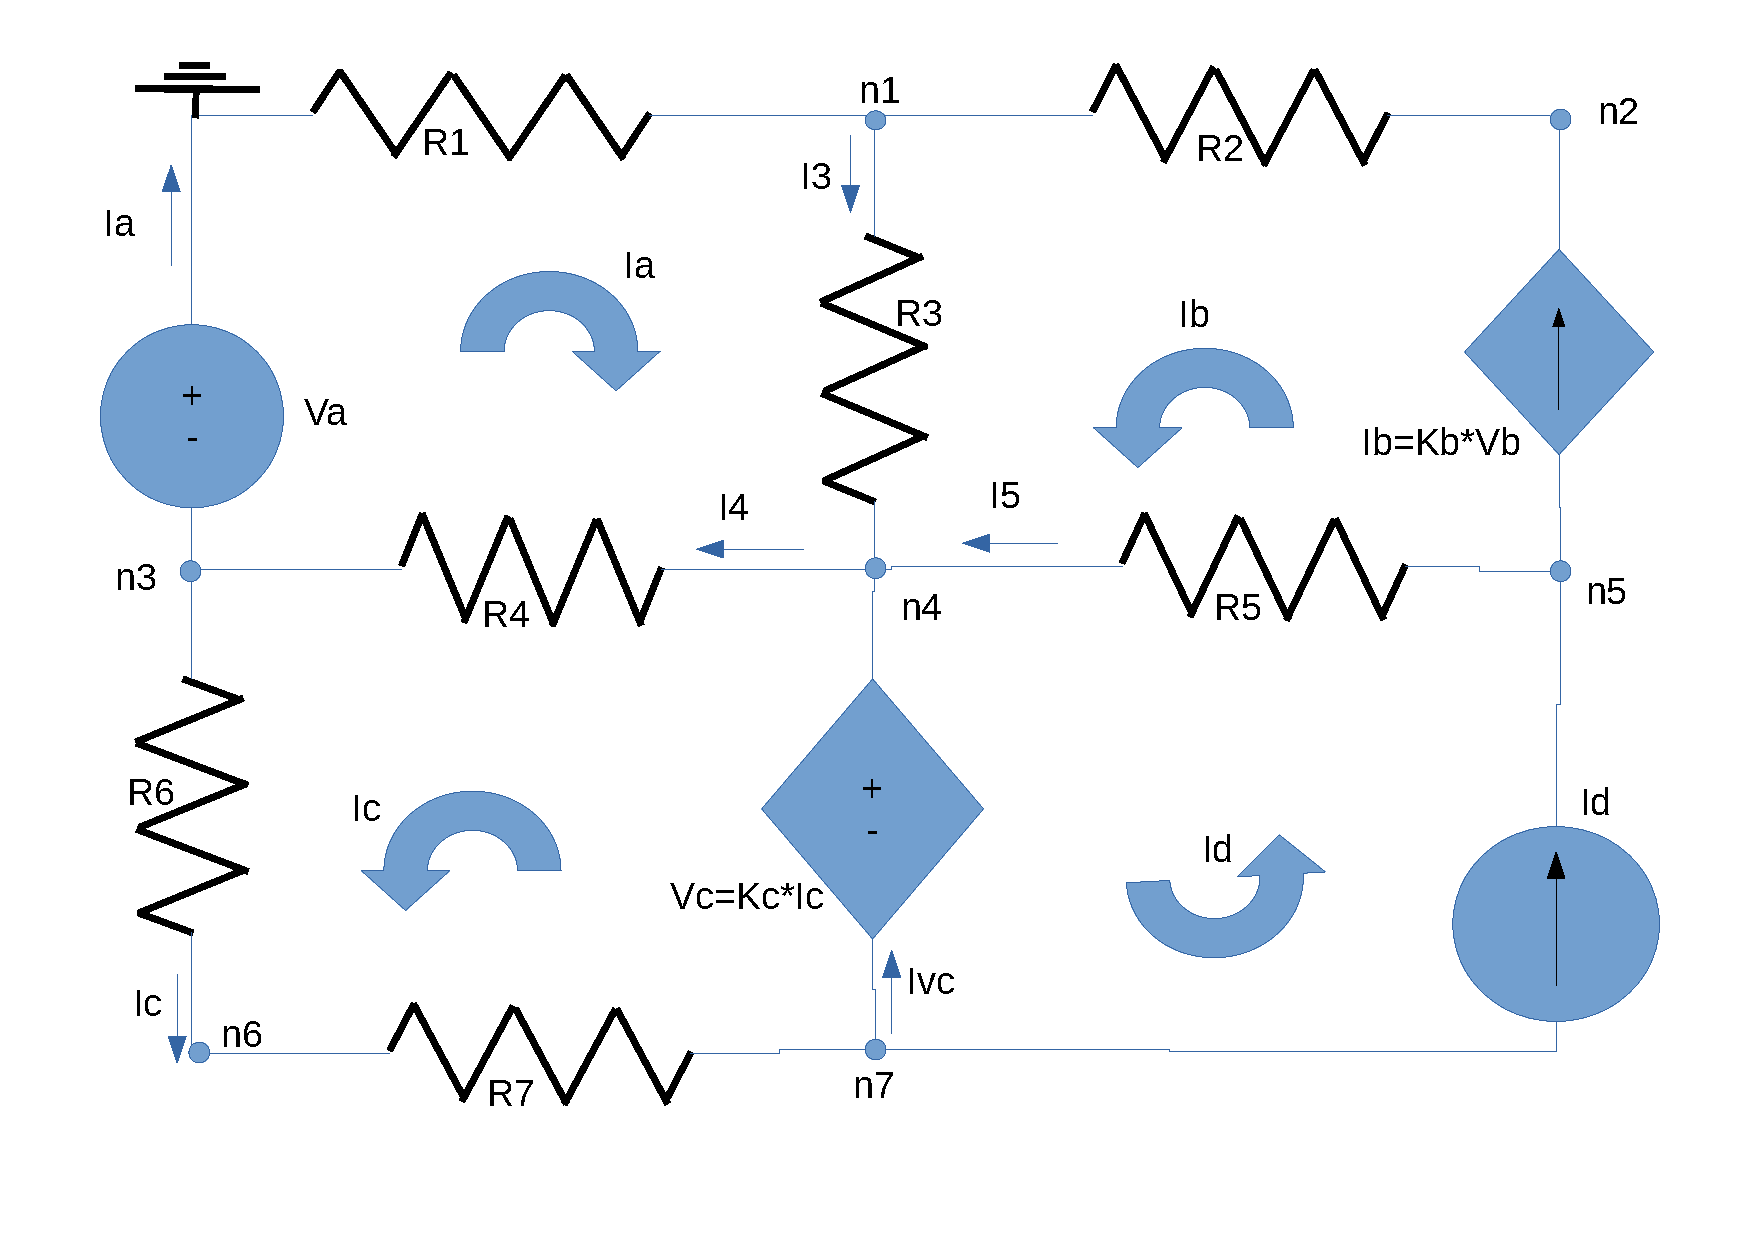
\includegraphics[width=0.7\linewidth]{circuit.pdf}
\caption{First laboratory circuit.}
\label{fig:circuit}
\end{figure}

